\subsection{Grobkonzept}

\subsection{Kurzeinführung in Bluetooth Low Energy}

\subsection{Aufbau des Bluetooth-Moduls}

\subsubsection{Bluetooth-Modul der Peripheriegeräte}

\subsection{Ein- und Ausgabeelemente des Dojos}

\subsubsection{Audiointerface -- wtv020sd.c}
Das Modul wtv020sd.c beinhaltet die Initialisierung und Ansteuerung des Audiochip Wtv020sd \cite{WTV020}. Die Kommunikation zum Audiointerface erfolgt über die Standard GPIO (General Purpose Input Output) des nRF52. Es werden die Pins: Reset, Busy, Clk und Data verwendet. Über das Audiointerface können die Audiofiles der SD-Karte gezielt Abgespielt, Pausiert und die Audioausgabe vermindert oder verstärkt werden (Mehr Details zum Hardwareaufbau im Kapitel \ref{}). Dabei handelt es sich um 16-Bit Befehle welche über ein SPI (synchroner serieller Datenbus) mit einer Geschwindigkeit von 5kHz gesendet werden.

\subsubsection{Peripherie -- ts3a27518e.c ts4871.c periphery.c }
Im Modul ts4871.c ist definiert mit welchem Pin der Audioverstärker ein- und ausgeschalten werden kann, in diesem Falle ist es der Standbypin (gem. Datenblat \cite{TS4871}). Des weiteren sind im Modul ts3a27518e.c die Pinausgänge für den Multiplexer, zwischen SD-Karte und Audiointerface definiert (gem. Datenblatt \cite{TS3A27518E}). Es kann zwischen Adio- und USB-Modus gewechselt werden.\\
Das Modul periphery.c beinhaltet die Verarbeitung der Tastereingaben und die Ausgabe des Feedbacks über den Vi1


\subsubsection{Peripherie -- ts3a27518e.c ts4871.c}

\subsection{Hauptprogrammablauf}


\subsection{Java Anwendung}

Um es dem Benutzer so einfach wie möglich zu machen, wurde eine Java Anwendung gestaltet, welche Audiodateien auf den Dojo übertragen kann. Dabei versucht die Anwendung im Prinzip nichts anderes als die SD-Karte im Dojo via USB-Schnittstelle zu erkennen und dann die Audiodateien auf die SD-Karte zu kopieren. Dabei werden die Audiodateien auch gleich so Umbenannt, dass sie zu den entsprechenden Beacons zugeordnet und abgespielt werden können. Da sich immer alle Audiodateien in allen Sprachen auf dem Dojo befinden müssen, muss dieser Schritt auch nur bei neu dazugekommenen Kunstobjekten wiederholt werden. Weiter kann mit der Java Anwendung benutzerspezifische Einstellungen wie Sprache und Zugangsreche übertragen werden. Dies geschieht jedoch im Gegensatz zu den Audiodateien über BLE, weshalb auch der entsprechende COM-Port von Anwender selektiert werden muss, sowie die BLE Transmitter Station eingesteckt sein muss.

\newpage

\begin{figure}[htb]
	\centering
	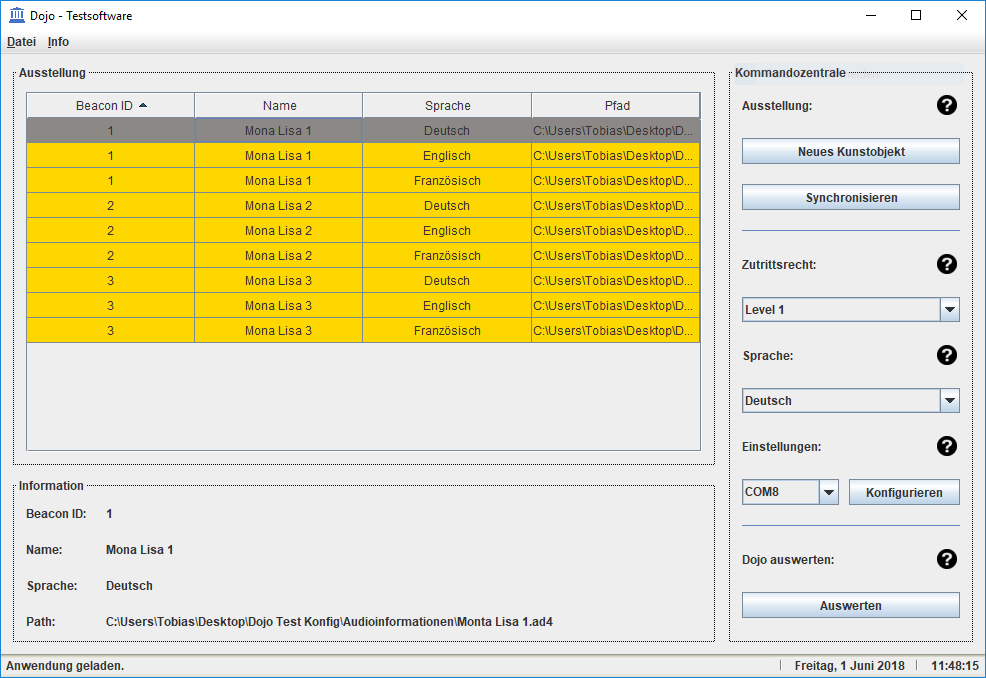
\includegraphics[width=\textwidth]{graphics/Java_Anwendung.png}
	\caption{Java Anwendung}
	\label{fig:Java Anwendung}
\end{figure}

Abbildung \ref{fig:Java Anwendung} zeigt die Java Anwendung, in der zurzeit gerade eine Ausstellung mit  drei Kunstobjekten (in allen drei Sprachen) geladen ist. Die Idee hinter dem Aufbau der Java Anwendung war, dass der Benutzer nichts falsch machen kann und auf falsche Aktionen entsprechend hingewiesen wird. Dies wurde schliesslich mittels treffenden Statusmeldungen unten links in der Statusbar umgesetzt.

\begin{figure}[htb]
	\centering
	
\includegraphics[width=\textwidth, height=5cm]{graphics/Dateiname.png}
	\caption{Dateiname Konventionen}
	\label{fig:Dateiname Konventionen}
\end{figure}


Abbildung \ref{fig:Dateiname Konventionen} wiederrum zeigt nach welchen Konventionen der Dateiname der Audioinformationen umbenannt wird, damit die Dateien von der Firmware erkannt und abgespielt werden kann.
